% !TeX encoding = UTF-8
% !TeX spellcheck = nl_NL
% !TeX TS-program = pdflate


%%%%%%%%%%%%%%%%%%%%%%%%%%%%%%%%%%%%%%%%%%%%%%%%%%%%%%%%%%%%%%%%%%%%%%%
%%
%%    COMMAND LINE ARGUMENTS IN C
%%
%%    (c)2017, J. op den Brouw <J.E.J.opdenBrouw@hhs.nl>
%%
%%    Version: 0.1
%%
%%%%%%%%%%%%%%%%%%%%%%%%%%%%%%%%%%%%%%%%%%%%%%%%%%%%%%%%%%%%%%%%%%%%%%%

\documentclass[a4paper,12pt,twoside]{article}

%% Set input encoding to UTF-8
\usepackage[utf8]{inputenc}
%% Use T1 output font encoding
\usepackage[T1]{fontenc}

%%
\usepackage{pict2e}

\usepackage{float}

%% Spelling
\usepackage[dutch]{babel}

%% Set page layout
\usepackage[a4paper,bindingoffset=0.2in,left=1.0in,right=1.0in,top=1.0in,bottom=1.4in,
                                                               footskip=0.5in]{geometry}
%% Using fancy headers and footers
%% http://ftp.snt.utwente.nl/pub/software/tex/macros/latex/contrib/fancyhdr/fancyhdr.pdf
\usepackage{fancyhdr}
\newcommand{\bookfancy}{
    \fancyhead{} % clear all header fields
    \fancyhead[LE,RO]{}
    %\fancyhead[RO,LE]{\thepage} % Right Odd, Left Even
    \fancyfoot{} % clear all footer fields
    \fancyfoot[LE,RO]{\thepage}   % page number in "outer" position of footer line
    \fancyfoot[RE,LO]{Command line argumenten en bestandsafhandeling in C} % other info in "inner" position of footer line
    \renewcommand{\headrulewidth}{0pt}
    \renewcommand{\footrulewidth}{0.4pt}
}
\pagestyle{fancy}
\bookfancy
\fancypagestyle{plain}{\bookfancy}

%% Use computer code listings
\usepackage{xcolor}
\usepackage{listings}
\usepackage{etoolbox}
\makeatletter
\patchcmd{\lsthk@SelectCharTable}{`)}{``}{}{}
\makeatother

%% Use textcomp for upright quotes in listings
\usepackage{textcomp}

\definecolor{dkgreen}{rgb}{0,0.6,0}
\definecolor{gray}{rgb}{0.5,0.5,0.5}
\definecolor{mauve}{rgb}{0.58,0,0.82}
\definecolor{lightgray}{rgb}{0.95,0.95,0.95}
\definecolor{GKYgray}{rgb}{0.65,0.65,0.65}
\definecolor{thuasgreen}{RGB}{158,167,0}
\definecolor{lightpink}{HTML}{F8E0E0}%{FBF3F3}%
%\definecolor{lightpink}{HTML}{F8E0E0}%{FBF3F3}%
\definecolor{cppgreen}{RGB}{0,160,0}
\definecolor{comment}{RGB}{128,128,255}
\definecolor{keyword}{RGB}{0,0,160}
\definecolor{number}{RGB}{240,0,240}
\definecolor{character}{RGB}{224,160,0}

\newcommand{\CodeSymbol}[1]{\textcolor{red}{#1}}
%% Define listing style for VHDL
\lstset{%
  language=C,
  basicstyle=\footnotesize\ttfamily,
  numbers=left,
  numberstyle=\tiny\color{gray},
  stepnumber=1,                           
  numbersep=8pt,
  keywordstyle=\bfseries\color{keyword},
  stringstyle=\color{blue},
%  keywords=[2]{printf,getchar,scanf,fflush,sqrt,pow,fib,faculteit,catalan,catalanRecursief,collatzSteps,f,leesGetal,max2,max5,gemiddelde,leesEnBerekenSom,leesCijfer,isisolatedprime,isprime,leesEnBerekenSom,leesEnBerekenMod9,reverse,strrev,is_palindroom,controleerNedEuroID,doorsnede,uniek,roll_dice,rand},
%  keywordstyle=[2]\color{orange},
%  keywords=[3]{<stdio.h>},
%  keywordstyle=[3]\color{orange},
%  keywords=[4]{main},
%  keywordstyle=[4]\color{purple},
  commentstyle=\itshape\color{comment},
  morecomment=[l][\color{cppgreen}]{\#},
%  backgroundcolor=\color{lightgray},
  showspaces=false,
  showstringspaces=false,
  showtabs=false,
  frame=lines,
  rulecolor=\color{black},
  tabsize=4,
  captionpos=b,
  breaklines=true,
  breakatwhitespace=false,
  title=\lstname,
  upquote=true,
  aboveskip=-1ex,
  belowskip=-2ex,
  literate=%
    *{0}{{{\textcolor{number}0}}}1
    {1}{{{\textcolor{number}1}}}1
    {2}{{{\textcolor{number}2}}}1
    {3}{{{\textcolor{number}3}}}1
    {4}{{{\textcolor{number}4}}}1
    {5}{{{\textcolor{number}5}}}1
    {6}{{{\textcolor{number}6}}}1
    {7}{{{\textcolor{number}7}}}1
    {8}{{{\textcolor{number}8}}}1
    {9}{{{\textcolor{number}9}}}1
    {\{}{{\CodeSymbol{\{}}}1
    {\}}{{\CodeSymbol{\}}}}1
    {(}{{\CodeSymbol{(}}}1
    {)}{{\CodeSymbol{)}}}1
    {>}{{\CodeSymbol{$>$}}}1
    {<}{{\CodeSymbol{$<$}}}1
    {=}{{\CodeSymbol{$=$}}}1
    {;}{{\CodeSymbol{$;$}}}1
    {,}{{\CodeSymbol{$,$}}}1
    {*}{{\CodeSymbol{$*$}}}1
    {+}{{\CodeSymbol{$+$}}}1
    {!}{{\CodeSymbol{!}}}1
    {\&}{{\CodeSymbol{\&}}}1,
    moredelim=[s][\textcolor{character}]{'}{'}
}

\usepackage{parskip}

%% Use the Charter and Nimbus Mono fonts
\usepackage[scaled=1.1]{nimbusmono}
\usepackage[bitstream-charter]{mathdesign}
%% Use microtype
\usepackage[stretch=10]{microtype}

%% Making captions nicer...
\usepackage[font=footnotesize,format=plain,labelfont=bf,textfont=sl]{caption}
\usepackage[labelformat=simple,font=footnotesize,format=plain,labelfont=bf,textfont=sl]{subcaption}
\captionsetup[figure]{format=hang,justification=centering,singlelinecheck=off,skip=2ex}
\captionsetup[table]{format=hang,justification=centering,singlelinecheck=off,skip=2ex}
\captionsetup[subfigure]{format=hang,justification=centering,singlelinecheck=off,skip=2ex}
\captionsetup[subtable]{format=hang,justification=centering,singlelinecheck=off,skip=2ex}
%% Put parens around the subfig name (a) (b) etc. Needs labelformat simple
\renewcommand\thesubfigure{(\alph{subfigure})}
\renewcommand\thesubtable{(\alph{subtable})}

\usepackage{graphicx}

\usepackage{mathtools}


\author{J.E.J. op den Brouw$^*$\thanks{$^*$De Haagse Hogeschool, \texttt{\footnotesize J.E.J.opdenBrouw@hhs.nl}, versie 1.1.}}
\title{Command line argumenten en bestandsafhandeling in C}

\begin{document}
%\raggedbottom
\maketitle

\section{Command line argumenten in C}
In besturingssystemen die C ondersteunen zoals Windows, Linux en Mac OS X, 
is het mogelijk om een C-programma \textsl{command line argumenten} mee te geven. In
dit document doen we dat in een zogenoemde DOS-box onder Windows. In figuur~\ref{fig:vbarg}
is te zien dat het programma \lstinline|myprog.exe| gestart wordt met de argumenten
\lstinline[literate=]|argument1| en \lstinline[literate=]|argument2|. Het programma drukt
eenvoudigweg alle argumenten op het beeldscherm af. Te zien is dat ook de programmanaam
als argument wordt meegegeven.

\begin{figure}[!ht]
\centering
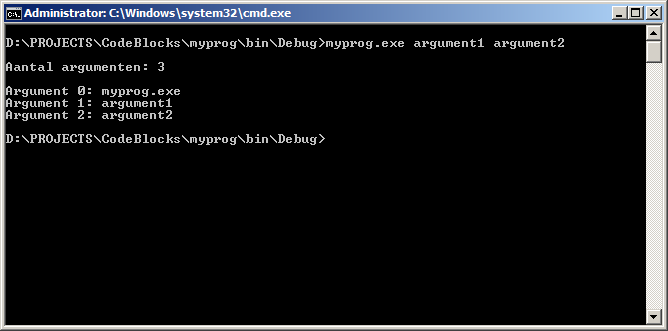
\includegraphics[width=\textwidth]{myprog.png}
\caption{Voorbeeld van een commando met argumenten.}
\label{fig:vbarg}
\end{figure}

%%%\begin{lstlisting}[caption=Voorbeeld van een commando met argumenten.,label=cod:vbarg]
%%%myprog.exe argument1 argument2
%%%\end{lstlisting}

Elk C-programma krijgt per definitie de twee parameters \lstinline|argc| en \lstinline|argv|
mee, die aan \lstinline|main()|
worden meegegeven. Dit is te zien in listing~\ref{cod:defsarg}.

\begin{figure}[!ht]
\begin{lstlisting}[caption=Declaratie van de command line parameters.,label=cod:defsarg]
int main(int argc, char *argv[]) {

    /* rest of the code */
    
    return 0;
}
\end{lstlisting}
\end{figure}

De integer \lstinline|argc| (\textbf{arg}ument \textbf{c}ount) geeft aan hoeveel
parameters aan het C-programma zijn meegegeven. De pointer \lstinline|*argv[]|
(\textbf{arg}ument \textbf{v}ector) is  een pointer naar een lijst van pointers
naar strings. Elke string bevat een argument. Per definitie wijst \lstinline|argv[0]|
naar een string waarin de programmanaam vermeld staat. Dat houdt in dat \lstinline|argc| dus minstens 1 is.
Er zijn dan geen optionele argumenten meegegeven.

In het voorbeeldprogramma is \lstinline|argc| dus 3 en zijn
\lstinline|argv[0]|, \lstinline|argv[1]| en \lstinline|argv[2]| pointers naar respectievelijk
\lstinline[literate=]|myprog.exe|, \lstinline[literate=]|argument1| en \lstinline[literate=]|argument2|. In
figuur~\ref{fig:argcargv} is een uitbeelding van de variabelen \lstinline|argc|
en \lstinline|argv| te zien. De strings worden, zoals gebruikelijk in C, afgesloten
met een \lstinline[literate=]|\0|-karakter. De C-standaard schrijft voor dat de lijst van strings
wordt afgesloten met een \lstinline|null|-adres.

\begin{figure}[!ht]
\centering
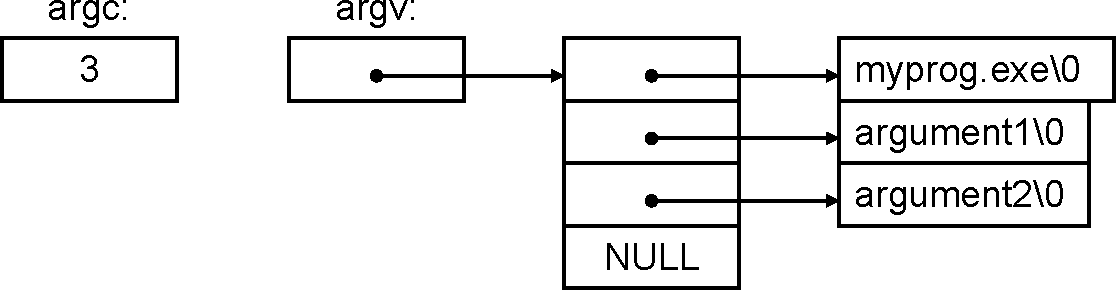
\includegraphics[scale=0.55]{argcargv.pdf}
\caption{Uitbeelding van de variabelen argc en argv.}
\label{fig:argcargv}
\end{figure}

Het programma \lstinline|myprog.exe| is te zien in listing~\ref{cod:myprogexe}. Het
programma drukt eerst de variabele \lstinline|argc| af. Met behulp van een \lstinline|for|-lus
worden de argumenten \'e\'en voor \'e\'en afgedrukt. Merk op dat \lstinline|argv[i]| een
pointer is naar het $i^e$ argument. We kunnen \lstinline|argv[i]| dus direct gebruiken
voor het afdrukken van de bijbehorende string.

\begin{figure}[H]
\begin{lstlisting}[caption=Het programma myprog.exe.,label=cod:myprogexe]
#include <stdio.h>
#include <stdlib.h>

int main(int argc, char *argv[]) {

    int i;

    printf("\nAantal argumenten: %d\n\n", argc);
    for (i = 0; i<argc; i++) {
        printf("Argument %d: %s\n", i, argv[i]);
    }
    return 0;
}
\end{lstlisting}
\end{figure}

\section{Bestandsafhandeling in C}
In C is het mogelijk om met bestanden op de harde schijf (of USB-stick of SD-card) te
werken. We spreken dan over File I/O.

In listing~\ref{cod:writefile} is de code te zien om een bestand te schrijven. We zullen
er stap voor stap doorheen lopen. In regel~6 wordt de pointer \lstinline|outfile| naar
een object \lstinline|FILE| gedeclareerd. Met behulp van de pointer kunnen we onder
andere lezen van een bestand en schrijven naar een bestand. In regel~8 wordt het
bestand \lstinline|C:\temp\testbestand.txt| geopend voor schrijven. Dat is te zien
aan de tweede argument \lstinline|"w"|. Merk op dat in de bestandsnaam gebruik is
gemaakt van een dubbele backslash omdat een backslash door C wordt gebruikt voor
afdrukbare karakters zoals \lstinline|\n|. De functie \lstinline|fopen| geeft een
adres terug die wordt toegekend aan de pointer \lstinline|outfile|. Als om \'e\'en
of andere reden het bestand niet geopend kan worden, geeft de functie \lstinline|fopen|
een \lstinline|null|-adres terug. We moeten hier natuurlijk op testen. Dat is te
zien in regel~10. We drukken dan een verklarende tekst af (regel~11). Als het
bestand voor schrijven geopend kan worden, dan schrijven we een regel naar dat
bestand. Dat is te zien regel~13. De functie \lstinline|fprintf| lijkt veel op de
bekende \lstinline|printf|-functie maar heeft \'e\'en extra parameter, namelijk
de pointer \lstinline|outfile|. In regel~14 wordt het bestand met behulp van de
functie \lstinline|fclose| gesloten.

\begin{figure}[H]
\begin{lstlisting}[caption=Voorbeeld schrijven naar een bestand.,label=cod:writefile]
#include <stdio.h>
#include <stdlib.h>

int main()
{
    FILE *outfile;

    outfile = fopen("C:\\temp\\testbestand.txt", "w");

    if (outfile == NULL) {
        printf("Bestand kan niet geopend worden.\n");
    } else {
        fprintf(outfile, "Een stukje tekst\n");
        fclose(outfile);
    }

    return 0;
}
\end{lstlisting}
\end{figure}

Listing~\ref{cod:readfile} laat de code zien om een bestand te lezen. Er wordt weer
gebruik gemaakt van een \lstinline|FILE|-pointer, in dit geval de pointer \lstinline|infile|.
Het genoemde bestand wordt weer geopend met de functie \lstinline|fopen| maar ditmaal
met als tweede argument \lstinline|"r"| wat staat voor lezen uit een bestand. Mocht
om \'e\'en of andere reden het bestand niet geopend kunnen worden, dan geeft
\lstinline|fopen| een \lstinline|null|-adres terug. Hier testen we op in regel~11.

In de regels 14 t/m 16 worden de karakters \'e\'en voor \'e\'en ingelezen en
afgedrukt op het beeldscherm. We zien hier een typische C-\lstinline|while|-constructie.
Er wordt
een karakter ingelezen door middel van de functie \lstinline|fgetc| en toegekend
aan de variabele \lstinline|ch|. Tegelijkertijd wordt getest of het ingelezen
karakter gelijk is aan \lstinline|EOF| wat staat voor end-of-file. Zolang dat niet
het geval is wordt het karakter afgedrukt met de functie \lstinline|printf|.

\begin{figure}[!t]
\begin{lstlisting}[caption=Voorbeeld lezen uit een bestand.,label=cod:readfile]
#include <stdio.h>
#include <stdlib.h>

int main()
{
    FILE *infile;
    int ch;

    infile = fopen("C:\\temp\\testbestand.txt", "r");

    if (infile == NULL) {
        printf("Kan bestand niet openen.");
    } else {
        while ((ch = fgetc(infile)) != EOF) {
            printf("%c", ch);
        }
    }
    
    fclose(infile);
    
    return 0;
}
\end{lstlisting}
\end{figure}

\section{Command line argumenten en bestandsafhandeling}
Het laatste voorbeeld betreft het kopi\"eren van een bestand. We gebruiken de
command line argumenten om de bestandsnamen door te geven en bestandsafhandeling
om het daadwerkelijke kopi\"eren te realiseren. Het programma is te vinden
in listing~\ref{cod:filecopy}.

We declareren eerst de pointers voor de twee bestanden, dit is te zien in regel~8.
In regel~10 declareren we twee integers, \'e\'en voor de in te lezen karakters en
\'e\'en voor het bijhouden hoeveel karakters er zijn gekopieerd. In de regels~14
t/m~17 testen we of het aantal opgegeven argumenten drie is. Zo niet, dan drukken
we een helptekst af om de gebruiker te informeren hoe het commando moet worden
gebruikt. Tevens wordt het programma afgesloten met een \lstinline|return|-statement.
Deze geeft de waarde $-1$ terug aan het besturingssysteem, een gebruikelijke techniek
in Unix-achtige omgevingen om foutmeldingen door te geven.

In de regels~20 t/m~23 wordt getest of de namen van de twee bestanden identiek zijn.
Dat mag natuurlijk niet anders wordt het leesbestand overschreven. We geven een
passende foutmelding en verlaten het programma middels een \lstinline|return|-statement
met de waarde~$-2$.

\begin{figure}[!p]
\begin{lstlisting}[caption=Programma om een bestand te kopi\"eren.,label=cod:filecopy]
#include <stdio.h>
#include <stdlib.h>
#include <string.h>

int main(int argc, char *argv[]) {

    /* The input and output file handlers */
    FILE *infile, *outfile;

    /* Character to read and character count */
    int ch, count = 0;

    /* We need exactly 3 arguments */
    if (argc != 3) {
        printf("Usage: %s infile outfile\n", argv[0]);
        return -1;
    }

    /* Test if input file and output file have the same name */
    if (strcmp(argv[1], argv[2]) == 0) {
        printf("Filenames cannot be the same\n");
        return -2;
    }

    /* Open the input file, exit if error */
    infile = fopen(argv[1], "r");
    if (infile == NULL) {
        printf("Cannot open input file %s\n", argv[1]);
        return -3;
    }

    /* Open the output file, exit if error */
    outfile = fopen(argv[2], "w");
    if (outfile == NULL) {
        printf("Cannot open output file %s\n", argv[2]);
        fclose(infile);
        return -4;
    }

    /* Copy characters from input file to output file */
    while ((ch = fgetc(infile)) != EOF) {
        count++;
        fprintf(outfile, "%c", ch);
    }

    printf("Copied %d characters\n", count);

    fclose(infile);
    fclose(outfile);

    return 0;
}
\end{lstlisting}
\end{figure}

In de regels~26 t/m 30 wordt het leesbestand geopend. We hebben dit al eerder besproken.
In de regels~33 t/m 38 wordt het schrijfbestand geopend. Ook dit is al eerder besproken.
Het daadwerkelijke kopi\"eren gebeurt in de regels~41 t/m 44. Tevens wordt bijgehouden
hoeveel karakters er zijn gekopieerd. Dit aantal wordt afgedrukt in regel~46.

We ronden het programma af door het leesbestand en schrijfbestand af te sluiten. Een
aantal voorbeelden van het gebruik van het programma is te zien in figuur~\ref{fig:filecopy}.

\begin{figure}[!ht]
\centering
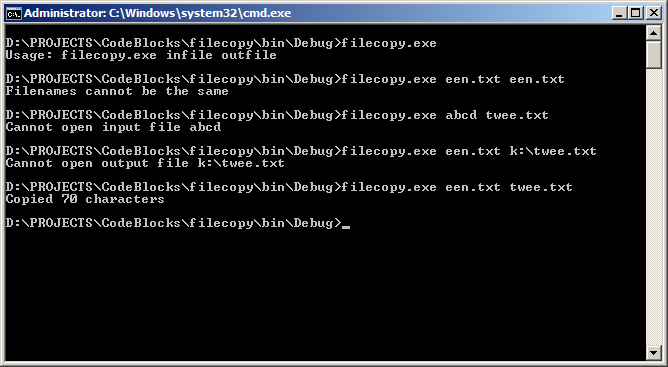
\includegraphics[width=\textwidth]{filecopy.png}
\caption{Voorbeelden van het kopieerprogramma.}
\label{fig:filecopy}
\end{figure}

\section{Openen van een DOS-box op Windows}
Een DOS-box kan je openen via de Start-knop (in het voorbeeld onder Windows 7).
Klik op Start en vul in het kader de tekst \lstinline|cmd.exe| in. Druk op de
enter-toets en een DOS-box wordt geopend. Zie figuur~\ref{fig:cmdexe}.

\begin{figure}[!ht]
\centering

\includegraphics[scale=0.63]{cmdexe.png}
\caption{Openen van een DOS-box.}
\label{fig:cmdexe}
\end{figure}

Vervolgens kun je navigeren naar de \textsl{executable} (uitvoerbaar programma)
middels het commando \lstinline|cd| (change directory). In het voorbeeld van
figuur~\ref{fig:filecopy} doe je als volgt:

\lstinline|cd \Users\JouwNaam\Documents\CodeBlocks\filecopy\bin\Debug|

Vul voor \lstinline|JouwNaam| je gebruikersnaam in waarmee je inlogt. We gaan er hier
trouwens vanuit dat je de programma's in de map \lstinline|CodeBlocks| zet die in de map
\lstinline|Documents| staat.

Als je je programma's op een andere schijf geplaatst hebt, moet je eerst van schijf veranderen.
Stel dat je je programma's op de \lstinline|D:|-schijf hebt geplaatst, dan verander je van
schijf met het commando:

\lstinline|D:|

Daarna kan je naar je map navigeren, bijvoorbeeld:

\lstinline|cd \PROJECTS\CodeBlocks\filecopy\bin\Debug|



\end{document}